\documentclass[letterpaper]{article}
\usepackage{fullpage}
\usepackage[utf8]{inputenc}
\usepackage{cite}
% \usepackage{breakurl}
\usepackage{xurl}
\usepackage{xcolor}
\usepackage{hyperref}
\hypersetup{
  colorlinks,
  linkcolor={green!80!black},
  citecolor={red!70!black},
  urlcolor={blue!70!black}
}
\usepackage[pdftex]{graphicx}
\usepackage[capitalize]{cleveref}
\usepackage{subcaption}
\usepackage{array}
\usepackage{xspace}
\usepackage{amssymb}

% Defs
\newcommand{\randomchoice}{\ensuremath{\stackrel{\$}{\leftarrow}}}
\newcommand{\Prob}[1]{{{\bf Pr}\left[\,{#1}\,\right]}}
\newcommand{\adv}{\ensuremath{\mathcal{A}}\xspace}
\newcommand{\gen}{\ensuremath{\mathsf{Gen}}}
\newcommand{\negl}{\nu}
\newcommand{\nonnegl}{\ensuremath{\tau}}
\newcommand{\secparam}{\ensuremath{\lambda}}
\newcommand{\fuzz}{\ensuremath{\mathsf{fuzz}}\xspace}
\newcommand{\dist}{\ensuremath{\mathsf{dist}}\xspace}
\newcommand{\compare}{\ensuremath{\mathsf{comp}}\xspace}
\newcommand{\attr}{\ensuremath{\mathsf{attr}}\xspace}
\newcommand{\zee}{\ensuremath{{\mathbb Z}}}
\newcommand{\maxdist}{\ensuremath{{\Delta_d}}}
\newcommand{\digest}{D}

\begin{document}

\begin{figure*}[t]
    \centering
    \begin{subfigure}[t]{0.48\linewidth}
    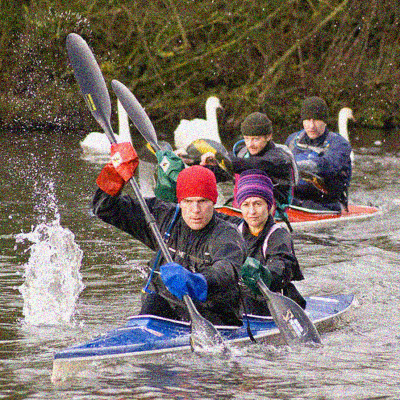
\includegraphics[width=0.48\textwidth]{figures/colgen_pdna_diff_1015.png}
    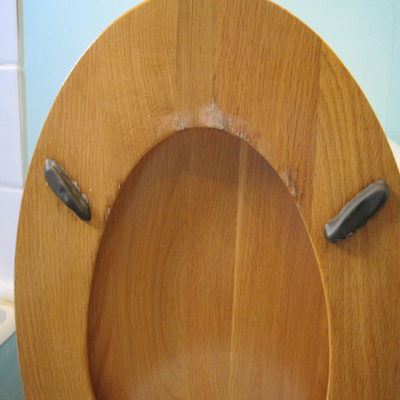
\includegraphics[width=0.48\textwidth]{figures/colgen_pdna_diff_target.png}
    \caption{PhotoDNA Collision at \maxdist = 1720}
    \label{fig:intro:fuzzy-gen:pdna}
    \end{subfigure}
    \begin{subfigure}[t]{0.48\linewidth}
    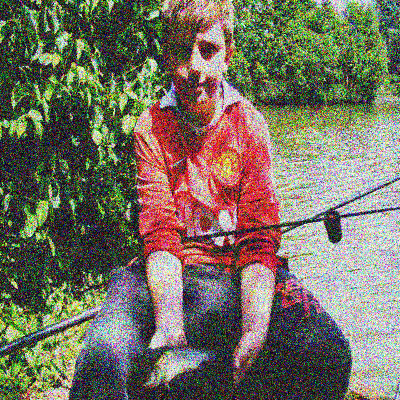
\includegraphics[width=0.48\textwidth]{figures/colgen_imgnet_pdq_boy2shark_250.png}
    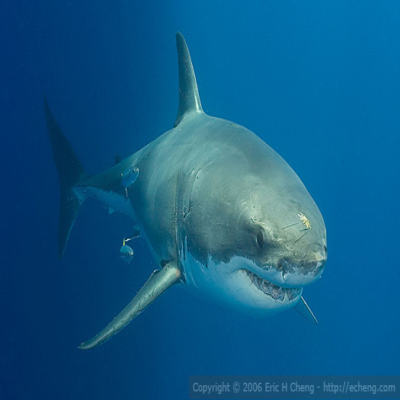
\includegraphics[width=0.48\textwidth]{figures/colgen_imgnet_pdq_boy2shark_target.png}
    \caption{PDQ Collision at \maxdist = 86}
    \label{fig:intro:fuzzy-gen:pdq}
    \end{subfigure}
    \begin{subfigure}[t]{0.48\linewidth}
    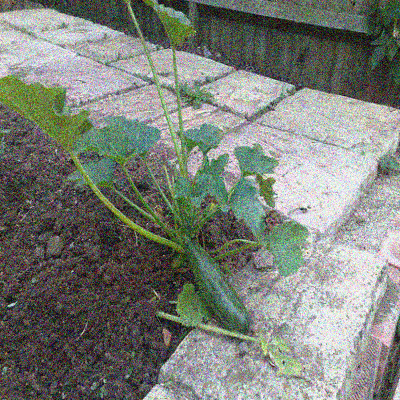
\includegraphics[width=0.48\textwidth]{figures/colgen_imgnet_pdna_best_20000.png}
    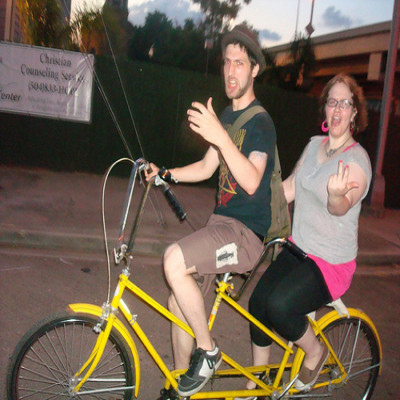
\includegraphics[width=0.48\textwidth]{figures/colgen_imgnet_pdna_best_target.png}
    \caption{PhotoDNA Collision at \maxdist = 342}
    \label{fig:intro:fuzzy-gen:pdna:best}
    \end{subfigure}
    \begin{subfigure}[t]{0.48\linewidth}
    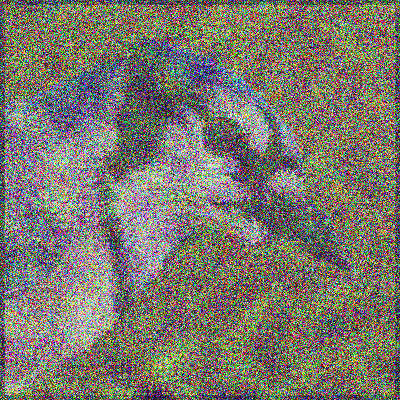
\includegraphics[width=0.48\textwidth]{figures/colgen_imgnet_pdq_egg_800.png}
    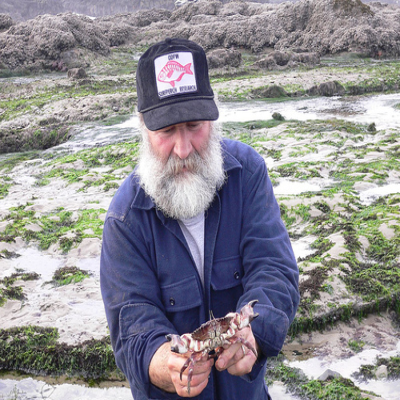
\includegraphics[width=0.48\textwidth]{figures/colgen_imgnet_pdq_egg_target.png}
    \caption{PDQ Collision at \maxdist = 38}
    \label{fig:intro:fuzzy-gen:pdq:best}
    \end{subfigure}
\end{figure*}

\end{document}
